% -*- latex -*-
%%%%%%%%%%%%%%%%%%%%%%%%%%%%%%%%%%%%%%%%%%%%%%%%%%%%%%%%%%%%%%%%
%%%%%%%%%%%%%%%%%%%%%%%%%%%%%%%%%%%%%%%%%%%%%%%%%%%%%%%%%%%%%%%%
%%%%
%%%% This text file is part of the source of slides for
%%%% `The Art of HPC, vol 1: The Science of Computing'
%%%% by Victor Eijkhout, copyright 2012-2024
%%%%
%%%%%%%%%%%%%%%%%%%%%%%%%%%%%%%%%%%%%%%%%%%%%%%%%%%%%%%%%%%%%%%%
%%%%%%%%%%%%%%%%%%%%%%%%%%%%%%%%%%%%%%%%%%%%%%%%%%%%%%%%%%%%%%%%

\Level 1 {Scalability analysis of dense matrix-vector product}

\frame{\frametitle{Parallel matrix-vector product; general}
  \begin{itemize}
  \item Assume a division by block rows
  \item Every processor $p$ has a set of row indices $I_p$
  \end{itemize}
  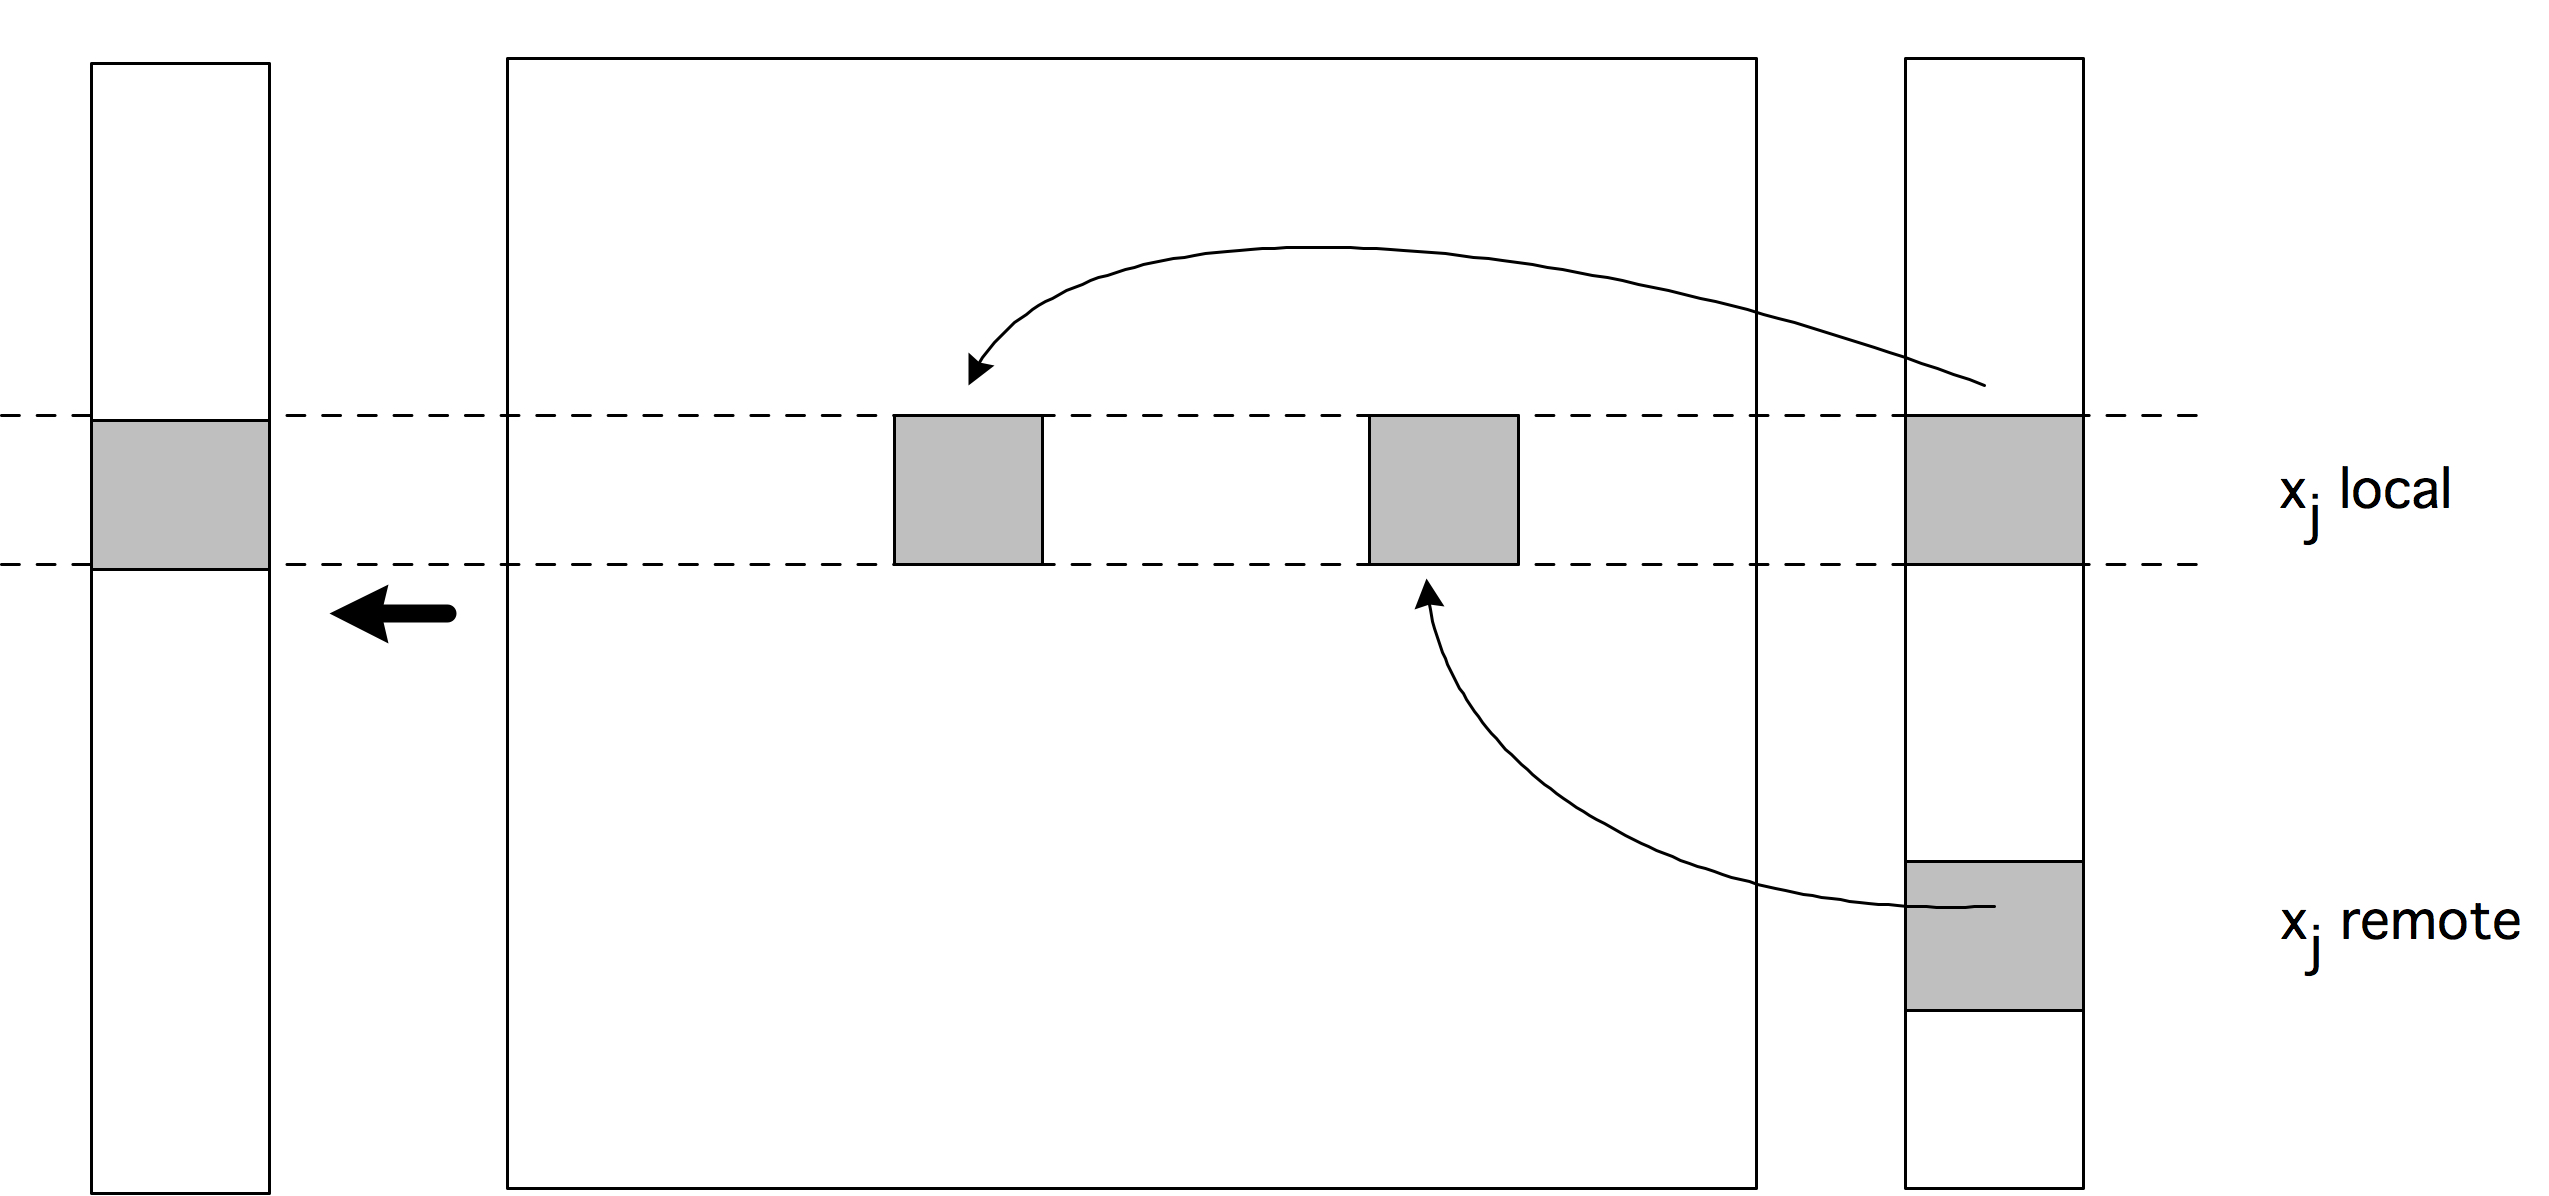
\includegraphics[scale=.06]{distmvp}
  Mvp on processor $p$:
  \[ \forall_{i\in I_p}\colon y_i=\sum_j a_{ij}x_j =\sum_q\sum_{j\in I_q} a_{ij}x_j \]
}

\frame{\frametitle{Local and remote operations}
Local and remote parts:

  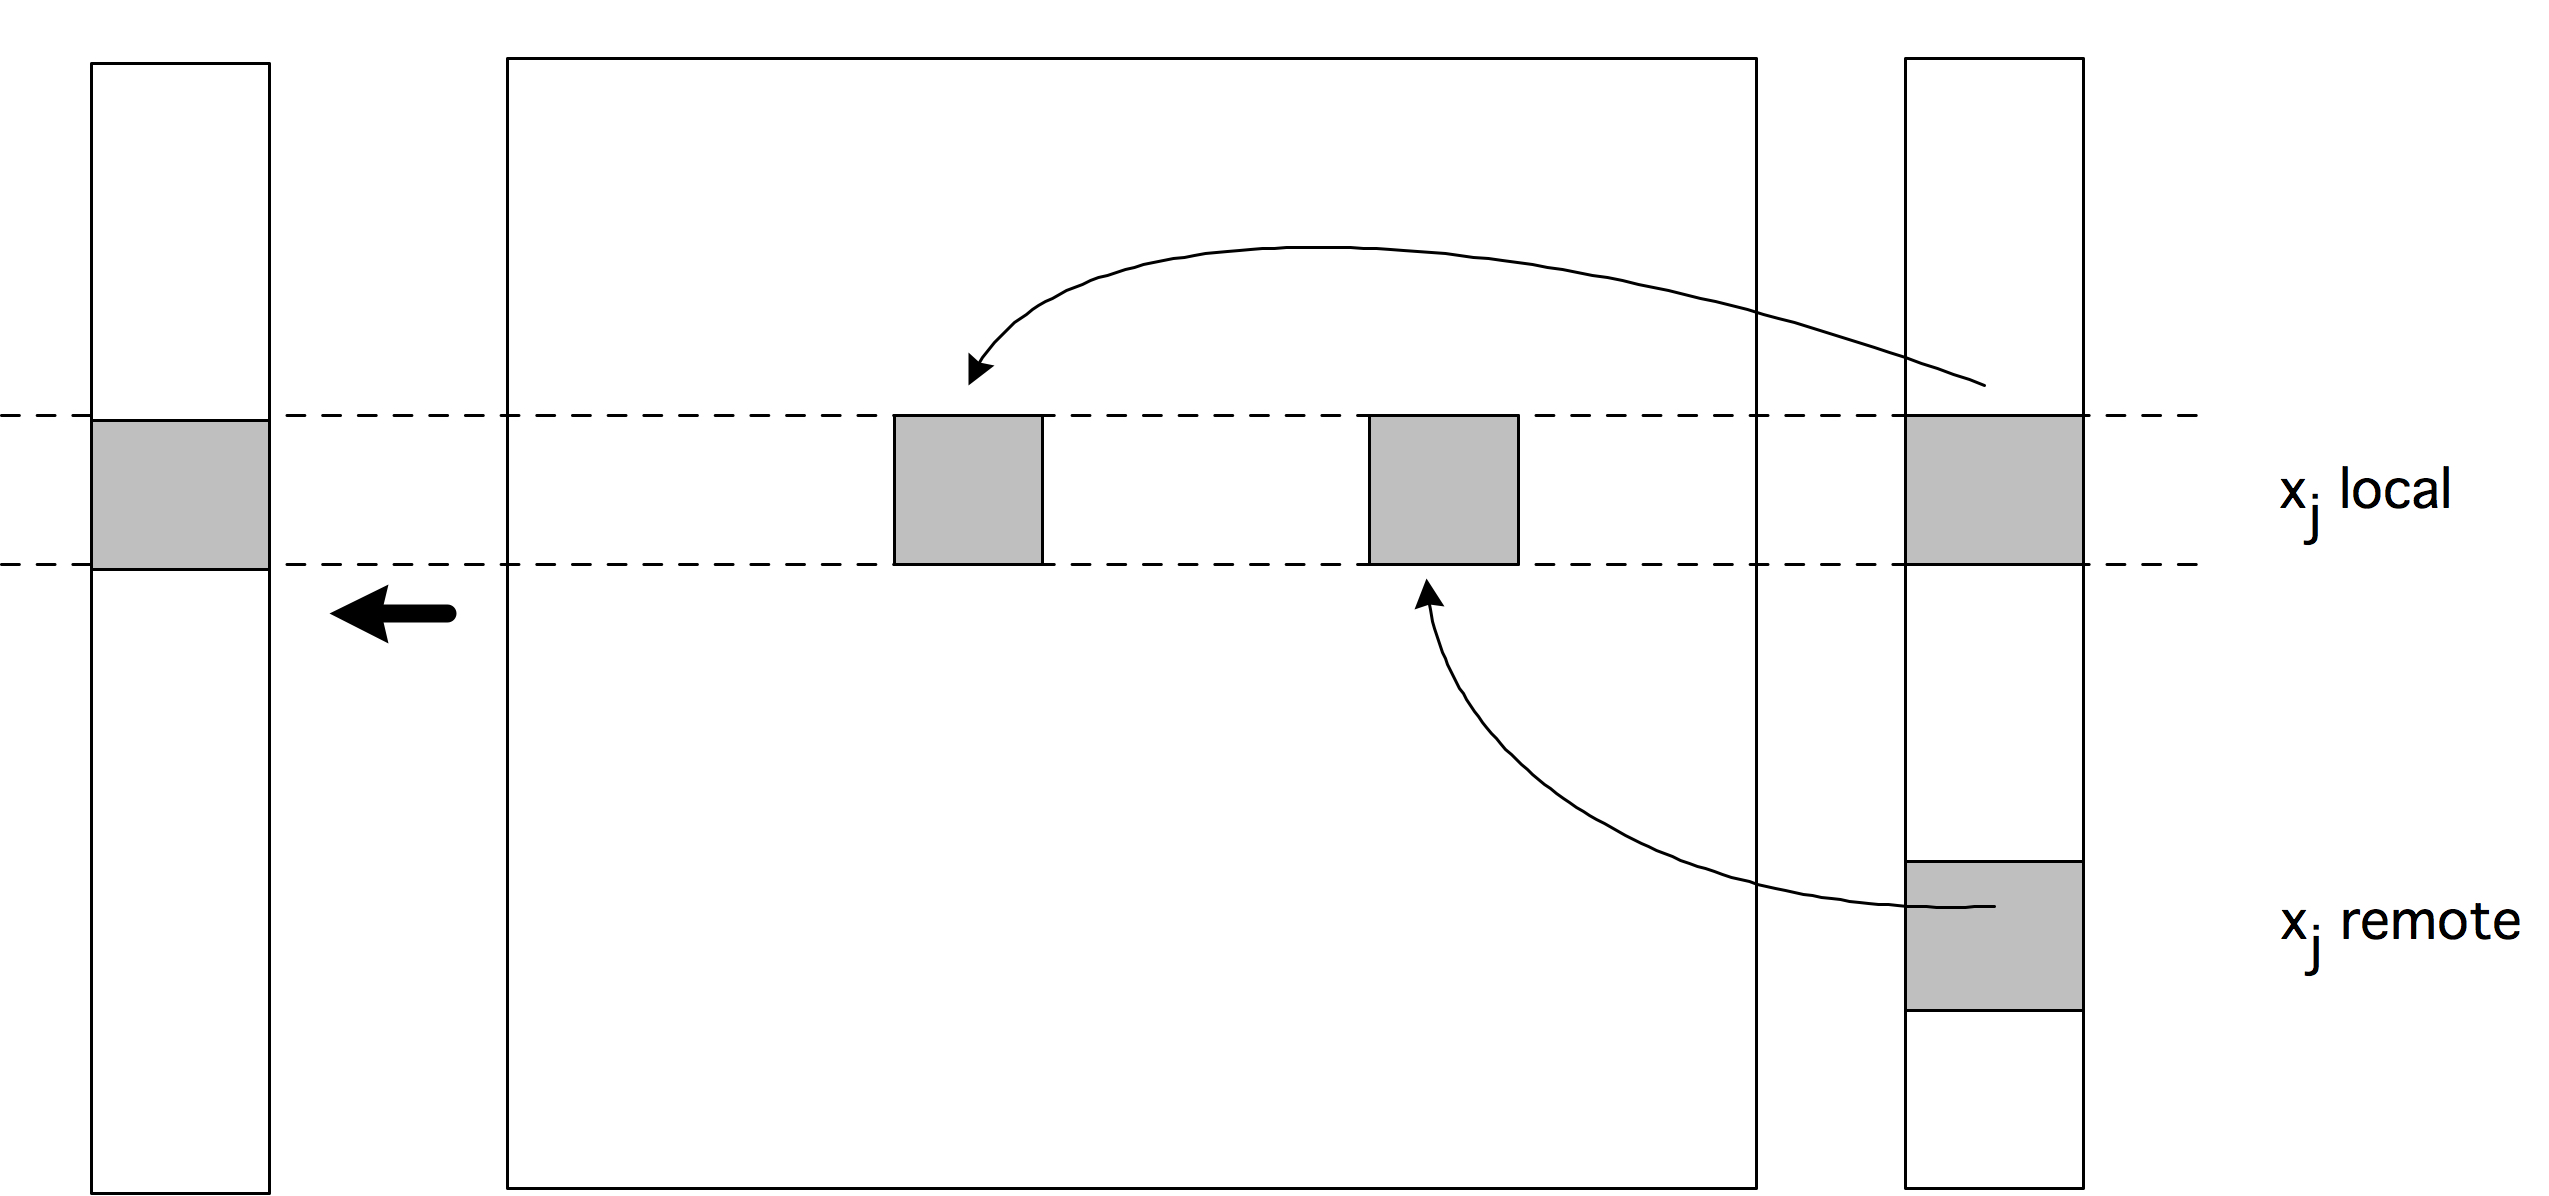
\includegraphics[scale=.06]{distmvp}

  \[ \forall_{i\in I_p}\colon y_i=\sum_{j\in
    I_p}a_{ij}x_j+\sum_{q\not=p}\sum_{j\in I_q} a_{ij}x_j 
  \]
  Local part $I_p$ can be executed right away, $I_q$ requires
  communication.
}

\begin{frame}{How to deal with remote parts}
  \begin{itemize}
  \item Very flexible: mix of working on local parts, and receiving remote parts.
  \item More orchestrated:
    \begin{enumerate}
    \item
      each process gets a full copy of the input vector (how?)
    \item then operates on the whole input
    \end{enumerate}
    Compare?
  \end{itemize}
  (Are we making a big assumption here?)
\end{frame}

\begin{frame}{Dense MVP}
\begin{itemize}
\item Separate communication and computation:
\item first allgather
\item then matrix-vector product
\end{itemize}
\end{frame}

\frame{\frametitle{Cost computation 1.}
Algorithm:
\begin{center}
\begin{tabular}{ p{2in}  p{2in}}\toprule
Step & Cost (lower bound) \\ \midrule
Allgather $ x_i $ so that $ x $ is available on all nodes & \\
Locally compute $ y_i = A_i x $ &
$ \approx 2 \frac{n^2}{P} \gamma $ \\ \bottomrule
\end{tabular}
\end{center}

}

\frame{\frametitle{Allgather}
Assume that data arrives over a binary tree:
\begin{itemize}
\item latency $\alpha\log_2 P$
\item transmission time, receiving $n/P$ elements from $P-1$ processors
\end{itemize}
}

\frame{\frametitle{}
Algorithm with cost:
\begin{center}
  \begin{tabular}{ p{2in} p{2in} }
    \toprule
Step & Cost (lower bound) \\ \midrule
Allgather $ x_i $ so that $ x $ is available on all nodes & 
$ \lceil \log_2(P)\rceil \alpha + \frac{P-1}{P} n \beta \approx
\log_2(P) \alpha + n \beta $ \\
Locally compute $ y_i = A_i x $ &
$ \approx 2 \frac{n^2}{P} \gamma $ \\
\bottomrule
\end{tabular}
\end{center}

}

\frame{\frametitle{Parallel efficiency}
Speedup:
\[
\begin{array}{rl}
  S_p^{\mbox{1D-row}}(n) &= 
  \frac{T_1(n)}{T_p^{\mbox{1D-row}}(n)} \\
  &=  \frac{2 n^2 \gamma}
        { 2 \frac{n^2}{p} \gamma + \log_2(p) \alpha + n \beta}\\
  & = \frac{p}
           { 1 + \frac{p \log_2(p)}{2 n^2} \frac{\alpha}{\gamma} 
               + \frac{p}{2 n} \frac{\beta}{\gamma} }\\
\end{array}
\]

Efficiency:
\[
\begin{array}{rl}
  E_p^{\mbox{1D-row}}(n) & = 
  \frac{S_p^{\mbox{1D-row}}(n)}{p}\\
  & = 
  \frac{1}
       { 1 + \frac{p \log_2(p)}{2 n^2} \frac{\alpha}{\gamma} 
         + \frac{p}{2 n} \frac{\beta}{\gamma} }.
\end{array}
\]

Strong scaling, weak scaling?
}

\frame{\frametitle{Optimistic scaling}
Processors fixed, problem grows:
\[
E_p^{\mbox{1D-row}}(n) = 
\frac{1}
{ 1 + \frac{p \log_2(p)}{2 n^2} \frac{\alpha}{\gamma} 
+ \frac{p}{2 n} \frac{\beta}{\gamma} }.
\]
Roughly $E_p\sim 1-n^{-1}$
}

\frame{\frametitle{Strong scaling}
Problem fixed, $p\rightarrow \infty$
\[
E_p^{\mbox{1D-row}}(n) = 
\frac{1}
{ 1 + \frac{p \log_2(p)}{2 n^2} \frac{\alpha}{\gamma} 
+ \frac{p}{2 n} \frac{\beta}{\gamma} }.
\]
\pause
Roughly $E_p\sim p^{-1}$
}

\frame{\frametitle{Weak scaling}
Memory fixed: \[ M=n^2/p \]
\[
E_p^{\mbox{1D-row}}(n) = 
\frac{1}
{ 1 + \frac{p \log_2(p)}{2 n^2} \frac{\alpha}{\gamma} 
+ \frac{p}{2 n} \frac{\beta}{\gamma} } =
\frac{1}
{ 1 + \frac{\log_2(p)}{2 M} \frac{\alpha}{\gamma} 
+ \frac{\sqrt p}{2 \sqrt M} \frac{\beta}{\gamma} }
\]
\pause
Does not scale: $E_p\sim 1/\sqrt p$\\
problem in $\beta$ term: too much communication
}

\frame{\frametitle{Two-dimensional partitioning}
{\tiny
\[ \kern-.25in
\begin{array}{| c | c | c | c |} \hline
% 0,0
\begin{array}{c c c c}
x_0\\
a_{00} & a_{01} &a_{02} & y_0\\
a_{10} & a_{11} &a_{12} & \\
a_{20} & a_{21} &a_{22} & \\
a_{30} & a_{31} &a_{32} & \\
\end{array}
&
% 0,1
\begin{array}{c c c c}
x_3\\
a_{03} & a_{04} &a_{05} & \\
a_{13} & a_{14} &a_{15} & y_1\\
a_{23} & a_{24} &a_{25} & \\
a_{33} & a_{34} &a_{35} & \\
\end{array}
&
% 0,2
\begin{array}{c c c c}
x_6\\
a_{06} & a_{07} &a_{08} & \\
a_{16} & a_{17} &a_{18} & \\
a_{26} & a_{27} &a_{28} & y_2 \\
a_{37} & a_{37} &a_{38} & \\
\end{array}
&
% 0,3
\begin{array}{c c c c}
x_9\\
a_{09} & a_{0,10} & a_{0,11} & \\
a_{19} & a_{1,10} & a_{1,11} & \\
a_{29} & a_{2,10} & a_{2,11} & \\
a_{39} & a_{3,10} & a_{3,11} & y_3 \\
\end{array}
\\ \hline
% 1,0
\begin{array}{c c c c}
& x_1\\
a_{40} & a_{41} &a_{42} & y_4\\
a_{50} & a_{51} &a_{52} & \\
a_{60} & a_{61} &a_{62} & \\
a_{70} & a_{71} &a_{72} & \\
\end{array}
&
% 1,1
\begin{array}{c c c c}
& x_4\\
a_{43} & a_{44} &a_{45} & \\
a_{53} & a_{54} &a_{55} & y_5\\
a_{63} & a_{64} &a_{65} & \\
a_{73} & a_{74} &a_{75} & \\
\end{array}
&
% 1,2
\begin{array}{c c c c}
& x_7\\
a_{46} & a_{47} &a_{48} & \\
a_{56} & a_{57} &a_{58} & \\
a_{66} & a_{67} &a_{68} & y_6 \\
a_{77} & a_{77} &a_{78} & \\
\end{array}
&
% 1,3
\begin{array}{c c c c}
& x_{10}\\
a_{49} & a_{4,10} & a_{4,11} & \\
a_{59} & a_{5,10} & a_{5,11} & \\
a_{69} & a_{6,10} & a_{6,11} & \\
a_{79} & a_{7,10} & a_{7,11} & y_7 \\
\end{array}
\\ \hline
% 0,0
\begin{array}{c c c c}
&&x_2\\
a_{80} &  a_{81} &  a_{82} & y_8\\
a_{90} &  a_{91}   &a_{92} & \\
a_{10,0} &a_{10,1} &a_{10,2} & \\
a_{11,0} &a_{11,1} &a_{11,2} & \\
\end{array}
&
% 0,1
\begin{array}{c c c c}
&&x_5\\
a_{83} &   a_{84} &  a_{85} & \\
a_{93} &   a_{94} &  a_{95} & y_9\\
a_{10,3} & a_{10,4} &a_{10,5} & \\
a_{11,3} & a_{11,4} &a_{11,5} & \\
\end{array}
&
% 0,2
\begin{array}{c c c c}
&&x_8\\
a_{86} &   a_{87} &  a_{88} & \\
a_{96} &   a_{97} &  a_{98} & \\
a_{10,6} & a_{10,7} &a_{10,8} & y_{10} \\
a_{11,7} & a_{11,7} &a_{11,8} & \\
\end{array}
&
% 0,3
\begin{array}{c c c c}
&&x_{11}\\
a_{89} &   a_{8,10} &  a_{8,11} & \\
a_{99} &   a_{9,10} &  a_{9,11} & \\
a_{10,9} & a_{10,10} & a_{10,11} & \\
a_{11,9} & a_{11,10} & a_{11,11} & y_{11} \\
\end{array}
\\ \hline
\end{array}
\]
}
}

\frame{\frametitle{Two-dimensional partitioning}
Processor grid $p=r\times c$, assume $r,c\approx\sqrt p$.

{\tiny
\[ \kern-.25in
\begin{array}{| c | c | c | c |} \hline
% 0,0
\begin{array}{c c c c}
x_0\\
a_{00} & a_{01} &a_{02} & y_0\\
a_{10} & a_{11} &a_{12} & \\
a_{20} & a_{21} &a_{22} & \\
a_{30} & a_{31} &a_{32} & \\
\end{array}
&
% 0,1
\begin{array}{c c c c}
x_3\\
\\
&&& y_1\\
\\
\\
\end{array}
&
% 0,2
\begin{array}{c c c c}
x_6\\
\\
\\
&&& y_2 \\
\\
\end{array}
&
% 0,3
\begin{array}{c c c c}
x_9\\
\\
\\
\\
&&& y_3 \\
\end{array}
\\ \hline
% 1,0
\begin{array}{c c c c}
\phantom{a_{00}}& x_1\uparrow\\
\phantom{a_{00}}&\phantom{a_{00}}&\phantom{a_{00}}& y_4\\
\\
\\
\\
\end{array}
&
% 1,1
\begin{array}{c c c c}
& x_4\\
\\
&&& y_5\\
\\
\\
\end{array}
&
% 1,2
\begin{array}{c c c c}
& x_7\\
\\
\\
&&& y_6 \\
\\
\end{array}
&
% 1,3
\begin{array}{c c c c}
& x_{10}\\
\\
\\
\\
&&& y_7 \\
\end{array}
\\ \hline
% 0,0
\begin{array}{c c c c}
\phantom{a_{00}}&\phantom{a_{00}}&x_2\uparrow\\
\phantom{a_{00}}&\phantom{a_{00}}&\phantom{a_{00}}& y_8\\
\\
\\
\\
\end{array}
&
% 0,1
\begin{array}{c c c c}
&&x_5\\
\\
&&& y_9\\
\\
\\
\end{array}
&
% 0,2
\begin{array}{c c c c}
&&x_8\\
\\
\\
&&& y_{10} \\
\\
\end{array}
&
% 0,3
\begin{array}{c c c c}
&&x_{11}\\
\\
\\
\\
&&&y_{11} \\
\end{array}
\\ \hline
\end{array}
\]
}
}

\begin{frame}{Key to the algorithm}
\begin{itemize}
\item Consider block $(i,j)$
\item it needs to multiply by the $x$s in column~$j$
\item it produces part of the result of row~$i$
\end{itemize}
\end{frame}

\frame{\frametitle{Algorithm}
\begin{itemize}
\item Collecting $x_j$ on each processor $p_{ij}$ by an
  \emph{allgather} inside the processor columns.
\item Each processor $p_{ij}$ then computes $y_{ij} = A_{ij}x_j$.
\item Gathering together the pieces $y_{ij}$ in each processor row to
  form~$y_i$, distribute this over the processor row: combine to form
  a \emph{reduce-scatter}.
\item Setup for the next $A$ or $A^t$ product
\end{itemize}
}

\frame{\frametitle{Analysis 1.}
  \begin{tabular}{ p{2in} p{2in} }
    \toprule
Step & Cost (lower bound) \\ \midrule
Allgather $ x_i $'s  within columns & 
$ \lceil \log_2(r)\rceil \alpha + \frac{r-1}{p} n \beta $ \\
& $\approx \log_2(r) \alpha + \frac{n}{c} \beta $ \\
Perform local matrix-vector multiply &
$ \approx 2 \frac{n^2}{p} \gamma $ \\ 
Reduce-scatter $ y_i $'s  within rows & \\ \bottomrule
\end{tabular}
}

\frame{\frametitle{Reduce-scatter}
%% {\footnotesize
%% \[
%% \begin{array}{|c|cccc|}
%% \hline
%%   &t=1&t=2&t=3\\ \hline
%% p_0&x_0^{(0)},x_1^{(0)},x_2^{(0)}\downarrow,x_3^{(0)}\downarrow
%%    &x_0^{(0:2:2)},x_1^{(0:2:2)}\downarrow
%%     \hphantom{x_0^{(0:2:2)},x_1^{(0:2:2)}\downarrow}
%%    &x_0^{(0:3)}
%%     \hphantom{x_3^{(0:3)}x_3^{(0:3)}x_3^{(0:3)}}\\
%% p_1&x_0^{(1)},x_1^{(1)},x_2^{(1)}\downarrow,x_3^{(1)}\downarrow
%%    &x_0^{(1:3:2)}\uparrow,x_1^{(1:3:2)}
%%     \hphantom{x_0^{(0:2:2)},x_1^{(0:2:2)}\downarrow}
%%    &\hphantom{x_3^{(0:3)}} x_1^{(0:3)}
%%     \hphantom{x_3^{(0:3)}x_3^{(0:3)}} \\
%% p_2&x_0^{(2)}\uparrow,x_1^{(2)}\uparrow,x_2^{(2)},x_3^{(2)}
%%    &\hphantom{x_0^{(0:2:2)},x_1^{(0:2:2)}\downarrow}
%%     x_2^{(0:2:2)},x_3^{(0:2:2)}\downarrow
%%    &\hphantom{x_3^{(0:3)}x_3^{(0:3)}} x_2^{(0:3)}
%%     \hphantom{x_3^{(0:3)}}\\
%% p_3&x_0^{(3)}\uparrow,x_1^{(3)}\uparrow,x_2^{(3)},x_3^{(3)}
%%    &\hphantom{x_0^{(0:2:2)},x_1^{(0:2:2)}\downarrow}
%%     x_0^{(1:3:2)}\uparrow,x_1^{(1:3:2)}
%%    &\hphantom{x_3^{(0:3)}x_3^{(0:3)}x_3^{(0:3)}}
%%     x_3^{(0:3)}\\
%% \hline
%% \end{array}
%% \]
%% }
Time:
\[ \lceil \log_2 p\rceil\alpha +\frac{p-1}pn(\beta+\gamma). \]
}

\frame{\frametitle{}
  \begin{tabular}{ p{2in} p{2in} }
    \toprule
Step & Cost (lower bound) \\ \midrule
Allgather $ x_i $'s  within columns & 
$ \lceil \log_2(r)\rceil \alpha + \frac{r-1}{p} n \beta $ \\
& $\approx\log_2(r) \alpha + \frac{n}{c} \beta $ \\
Perform local matrix-vector multiply &
$ \approx 2 \frac{n^2}{p} \gamma $ \\ 
Reduce-scatter $ y_i $'s  within rows & 
$ \lceil \log_2(c)\rceil \alpha + \frac{c-1}{p} n \beta + \frac{c-1}{p} n \gamma $\\
& $ \approx \log_2(c) \alpha + \frac{n}{r} \beta + \frac{n}{r} \gamma $ \\
\bottomrule
\end{tabular}
}

\frame{\frametitle{Efficiency}
Let $r=c=\sqrt p$, then
\[
E_p^{\sqrt{p} \times \sqrt{p}}(n) = 
\frac{1}
{ 1 + \frac{p \log_2(p)}{2 n^2} \frac{\alpha}{\gamma} 
+ \frac{\sqrt{p}}{2n}\frac{
\left( 2 \beta + \gamma \right)}{\gamma}}
\]
}

\frame{\frametitle{Strong scaling}
Same story as before for $p\rightarrow\infty$:
\[
E_p^{\sqrt{p} \times \sqrt{p}}(n) = 
\frac{1}
{ 1 + \frac{p \log_2(p)}{2 n^2} \frac{\alpha}{\gamma} 
+ \frac{\sqrt{p}}{2n}\frac{
\left( 2 \beta + \gamma \right)}{\gamma}}
\sim p^{-1}
\]
No strong scaling
}

\frame{\frametitle{Weak scaling}
Constant memory $M=n^2/p$:
\only<1>{ \[
E_p^{\sqrt{p} \times \sqrt{p}}(n) = 
\frac{1}
{ 1 + \frac{p \log_2(p)}{2 n^2} \frac{\alpha}{\gamma} 
+ \frac{\sqrt{p}}{2n}\frac{
\left( 2 \beta + \gamma \right)}{\gamma}}
\phantom{ =
\frac{1}
{ 1 + \frac{ \log_2(p)}{2 M} \frac{\alpha}{\gamma} 
+ \frac{1}{2\sqrt M}\frac{
\left( 2 \beta + \gamma \right)}{\gamma}} }
\]}
\only<2->{ \[
E_p^{\sqrt{p} \times \sqrt{p}}(n) = 
\frac{1}
{ 1 + \frac{p \log_2(p)}{2 n^2} \frac{\alpha}{\gamma} 
+ \frac{\sqrt{p}}{2n}\frac{
\left( 2 \beta + \gamma \right)}{\gamma}}
=
\frac{1}
{ 1 + \frac{ \log_2(p)}{2 M} \frac{\alpha}{\gamma} 
+ \frac{1}{2\sqrt M}\frac{
\left( 2 \beta + \gamma \right)}{\gamma}}
\]}
\only<3>{
Weak scaling:\\
for $p\rightarrow\infty$ this is $\approx 1/\log_2 p$:\\
only slowly decreasing. }
}

\frame{\frametitle{LU factorizations}
\begin{itemize}
\item Needs a cyclic distribution
\item This is very hard to program, so:
\item Scalapack, 1990s product, not extendible, impossible interface
\item Elemental: 2010s product, extendible, nice user interface (and it is way faster)
\end{itemize}
}

